\section{Kiến thức nền tảng}
\label{sec:background}

\subsection{Directional Filter Bank (DFB)}

DFB được đề xuất bởi Bamberger và Smith \cite{bamberger1992} như một 2D filter bank có khả năng phân tích mặt phẳng tần số 2D thành các vùng hình nêm theo hướng (directional wedges). Không giống DWT chỉ cho ra ba hướng cố định (horizontal, vertical, diagonal), DFB có thể tạo ra $N$ subband tương ứng với $N$ hướng phân bố đều trong khoảng $[0°, 180°)$, với $N$ là lũy thừa của 2.

\textbf{Cấu trúc tree.}
Để đạt được $N = 2^l$ directional subband, DFB sử dụng một cây nhị phân (binary tree) $l$ tầng. Tại mỗi nút của cây, một 2-channel filter bank tách tín hiệu đầu vào thành hai subband, sau đó mỗi subband lại tiếp tục được tách ở tầng tiếp theo. Với $l = 3$ tầng, ta thu được 8 directional subband như trong paper của Rosiles và Smith \cite{rosiles2000}.

\textbf{Diamond filter và quincunx sampling.}
Mỗi 2-channel filter bank trong cây DFB sử dụng một cặp lowpass/highpass filter có passband hình thoi (diamond-shaped) trong miền tần số 2D. Việc downsampling sau mỗi tầng được thực hiện theo mạng quincunx (quincunx lattice), xác định bởi ma trận lấy mẫu:

\begin{equation}
    \mathbf{Q}_1 = \begin{bmatrix} 1 & 1 \\ 1 & -1 \end{bmatrix}, \qquad
    \mathbf{Q}_2 = \begin{bmatrix} 1 & -1 \\ 1 & 1 \end{bmatrix}
\end{equation}

Hai ma trận này có $|\det| = 2$, tức là mỗi lần downsampling giữ lại một nửa số pixel, tại các vị trí $(i, j)$ thỏa mãn $(i + j) \bmod 2 = 0$ (checkerboard pattern). Nhờ quincunx sampling kết hợp với diamond filter, DFB đạt được critically-sampled representation: tổng số hệ số ở tất cả các subband bằng đúng số pixel của ảnh gốc.

\textbf{Fan filter và modulation.}
Tại mỗi tầng của cây, diamond filter được biến đổi thành fan filter thông qua phép modulation — nhân tín hiệu với chuỗi $(-1)^{n_1 + n_2}$ hoặc các biến thể tương đương. Sự kết hợp giữa fan filter và quincunx sampling tạo ra các subband có passband dạng wedge trong mặt phẳng tần số: mỗi wedge tương ứng với một dải hướng nhất định. Hình~\ref{fig:dfb_partition} minh họa sự phân chia mặt phẳng tần số thành 8 wedge của một DFB 8 band.

\begin{figure}[H]
    \centering
    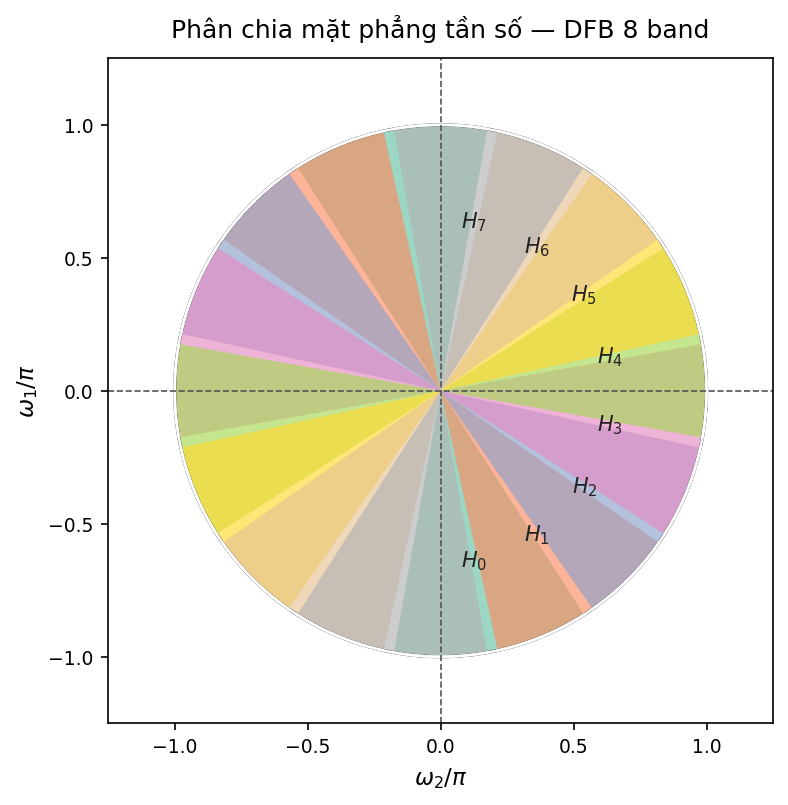
\includegraphics[width=0.6\textwidth]{figures/dfb_frequency_partition.png}
    \caption{Phân chia mặt phẳng tần số 2D thành 8 directional subband của DFB.
             Mỗi màu đại diện cho một wedge-shaped subband tương ứng với một hướng trong $[0°, 180°)$.}
    \label{fig:dfb_partition}
\end{figure}

\textbf{Perfect reconstruction.}
Nhờ thiết kế đối xứng của analysis và synthesis filter, DFB đảm bảo perfect reconstruction: khi không có bất kỳ biến đổi nào trên các subband, tín hiệu tái tạo hoàn toàn bằng tín hiệu gốc. Đây là tính chất quan trọng để đảm bảo chất lượng denoising.

% -----------------------------------------------------------------------
\subsection{Mô hình nhiễu và bài toán denoising}

Ta giả sử mô hình nhiễu cộng Gaussian (Additive White Gaussian Noise --- AWGN):

\begin{equation}
    y[n] = x[n] + \varepsilon[n], \qquad \varepsilon[n] \sim \mathcal{N}(0,\, \sigma^2)
\end{equation}

trong đó $y$ là ảnh quan sát được, $x$ là ảnh gốc cần khôi phục, và $\sigma$ là độ lệch chuẩn của nhiễu. Bài toán denoising là tìm ước lượng $\hat{x}$ từ $y$ sao cho giảm thiểu mean squared error (MSE):

\begin{equation}
    \text{MSE} = \frac{1}{N} \sum_{n} \bigl(\hat{x}[n] - x[n]\bigr)^2
\end{equation}

Trong miền transform, mỗi hệ số của subband $y_k = x_k + \varepsilon_k$ được xử lý độc lập bằng một hàm thresholding, sau đó tái tạo ảnh qua inverse transform.

% -----------------------------------------------------------------------
\subsection{Các phương pháp ước lượng threshold}

\subsubsection{Soft thresholding}

Soft thresholding (shrinkage) được định nghĩa là:

\begin{equation}
    \eta_t(y) = \operatorname{sign}(y) \cdot \max\!\bigl(|y| - t,\ 0\bigr)
\end{equation}

Các hệ số có $|y| \leq t$ bị đưa về 0 (loại bỏ noise), trong khi các hệ số lớn hơn được co lại về phía 0 một lượng $t$. So với hard thresholding $\hat{x} = y \cdot \mathbf{1}_{|y|>t}$, soft thresholding cho ra kết quả smoother do không tạo ra discontinuity tại $t$.

\subsubsection{SURE (Stein's Unbiased Risk Estimate)}

SURE cung cấp một ước lượng không chệch (unbiased estimate) của MSE mà không cần biết tín hiệu gốc $x$. Với $z_i = y_i/\sigma$ (chuẩn hóa về noise variance bằng 1), SURE cho soft threshold $\tilde{t} = t/\sigma$ là:

\begin{equation}
    \text{SURE}(\tilde{t})
    = n
    - 2 \cdot \#\{i : |z_i| \leq \tilde{t}\}
    + \sum_{i} \min\!\bigl(z_i^2,\ \tilde{t}^2\bigr)
    \label{eq:sure}
\end{equation}

Threshold tối ưu $t^* = \tilde{t}^* \cdot \sigma$ thu được bằng cách minimize \eqref{eq:sure} trên tập các giá trị $|z_i|$ đã được sắp xếp, với độ phức tạp $O(n \log n)$. Điểm mạnh của SURE là hoàn toàn data-driven --- không cần giả định prior về phân phối của tín hiệu.

\subsubsection{GCV (Generalised Cross Validation)}

GCV là một tiêu chí cross-validation tổng quát cho phép chọn threshold mà không cần biết $\sigma$. Trong miền chuẩn hóa $z_i = y_i/\sigma$:

\begin{equation}
    \text{GCV}(\tilde{t})
    = \frac{\displaystyle\sum_{i} \min\!\bigl(z_i^2,\ \tilde{t}^2\bigr)}
           {\!\left(\dfrac{\#\{|z_i| \leq \tilde{t}\}}{n}\right)^{\!2}}
    \label{eq:gcv}
\end{equation}

Tử số đo lường residual sum of squares sau khi threshold; mẫu số phạt theo tỷ lệ hệ số được giữ lại. GCV có xu hướng chọn threshold nhỏ hơn SURE trong một số trường hợp, dẫn đến denoising ít aggressive hơn.

\subsubsection{MAD (Median Absolute Deviation)}

MAD là phương pháp ước lượng $\sigma$ từ dữ liệu, robust với outlier:

\begin{equation}
    \hat{\sigma} = \frac{\operatorname{median}(|y|)}{0.6745}
\end{equation}

Hệ số $0.6745$ là median của $|\mathcal{N}(0,1)|$. Trong thực tế, $\hat{\sigma}$ được ước lượng từ subband tần số cao nhất --- nơi tín hiệu sparse nhất và noise chiếm ưu thế --- rồi áp dụng universal threshold của Donoho--Johnstone \cite{donoho1995}:

\begin{equation}
    t^* = \hat{\sigma}\,\sqrt{2\log n}
    \label{eq:universal}
\end{equation}

Universal threshold đảm bảo loại bỏ hoàn toàn noise với xác suất cao khi $n \to \infty$, nhưng thường quá conservative (threshold quá lớn) dẫn đến over-smoothing.

% -----------------------------------------------------------------------
\subsection{DWT-based denoising (Baseline)}

Wavelet thresholding là phương pháp baseline phổ biến nhất cho bài toán denoising. Pipeline gồm ba bước:
\begin{enumerate}
    \item Áp dụng multi-level 2D DWT để thu được các detail subband tại nhiều scale (horizontal, vertical, diagonal) và một approximation subband.
    \item Áp dụng threshold cho từng detail subband; giữ nguyên approximation subband.
    \item Tái tạo ảnh bằng inverse DWT.
\end{enumerate}

BayesShrink \cite{chang2000} là một trong những threshold estimator hiệu quả nhất cho DWT. Giả sử signal có prior Laplacian, threshold tối ưu cho từng subband là:

\begin{equation}
    t^* = \frac{\sigma^2}{\sigma_x}, \qquad
    \sigma_x = \sqrt{\max\!\bigl(\sigma_y^2 - \sigma^2,\ 0\bigr)}
    \label{eq:bayesshrink}
\end{equation}

trong đó $\sigma_y^2 = \operatorname{var}(y)$ là phương sai quan sát được của subband, $\sigma^2$ là noise variance, và $\sigma_x$ là ước lượng signal standard deviation. Ưu điểm của BayesShrink là cho threshold nhỏ ở các subband giàu tín hiệu (preserve edges) và threshold lớn ở các subband chủ yếu là noise (aggressive denoising).

Hạn chế căn bản của DWT là chỉ cung cấp ba hướng phân tích cố định ở mỗi scale. Điều này không đủ để biểu diễn sparse các cấu trúc hướng phức tạp, là động lực trực tiếp để sử dụng DFB trong bài toán denoising.
